\chapter{Fundamentação Teórica}

%%%%%%%%%%%%%%%%%%%%%%%%%%%%%%%%%%%%%%%%%%%%%%%%%%%%%%%%%%%%%%%%%%%%%%%%%%%%%%%%%%%%%%%%%%%%%%
\section {BIM}

O BIM (\textit{Building Information Modeling}, ou Modelagem da Informação da Construção) não é uma tecnologia específica, mas sim um processo integrado ao planejamento e execução de construções. De acordo com \citeonline{penttila2016}, o BIM consiste em um conjunto estruturado de políticas, processos e ferramentas que formam uma metodologia para gerenciar os dados digitais e os projetos de construção ao longo do ciclo de vida do edifício.

Esse recurso surgiu "após a inovação do CAD 3D paramétrico", tecnologia que foi amplamente adotada em setores como aeroespacial, automotivo e de manufatura \cite{monteiro2011}. O BIM vai além de representações tridimensionais que incluem dimensões, volumes e áreas, incorporando informações adicionais, como acabamento, custos, fabricantes e relações com outros elementos. Isso permite extrair informações de maneira mais eficiente e, em caso de alterações estruturais, atualizar todos os dados do projeto de forma centralizada. Apesar de seu caráter inovador, a implementação do BIM demanda equipes bem preparadas, tanto na etapa de controle quanto na de acompanhamento, o que pode elevar o custo inicial, embora proporcione uma gestão mais eficiente durante todo o ciclo de vida da construção \cite{coelho2018}.

Entre os principais benefícios do BIM está a possibilidade de trabalhar com várias dimensões em um único projeto. Com base nas informações adicionadas ao modelo, é possível reduzir falhas, otimizar prazos e garantir maior controle sobre as atualizações \cite{parreira2013}.

Segundo \cite{eastman2011}, o BIM possui sete dimensões que podem ser exploradas independentemente, desde que o modelo 3D já esteja desenvolvido. Isso significa, por exemplo, que uma análise 6D pode ser realizada sem a necessidade de uma inspeção 4D, como ilustrado na Figura \ref{img:3.1.1}.

\begin{itemize}

\item \textbf{BIM 3D - Modelo Virtual 3D}: Ampliando o conceito de modelagem 2D, o BIM 3D permite a visualização completa dos elementos em três dimensões (X, Y e Z), além de identificar colisões utilizando algoritmos originados da computação gráfica. Essa funcionalidade reduz significativamente custos na fase de design e na execução da obra.

\item \textbf{BIM 4D - Programação}: Esta dimensão organiza o modelo 3D em etapas, atribuindo sequências de montagem aos elementos. Além de possibilitar a visualização das fases do projeto, ela permite simular cronogramas e planejar prazos de entrega com maior precisão.

\item \textbf{BIM 5D - Estimativa de Custos}: Proporciona uma rápida estimativa de custos para diferentes fases do projeto, gerando relatórios financeiros e permitindo comparar alternativas em termos de tempo de execução e investimentos.

\item \textbf{BIM 6D - Sustentabilidade}: Essa dimensão possibilita integrar informações relacionadas à proteção ambiental e ao consumo de energia, otimizando os custos e investimentos durante e após a construção.

\item \textbf{BIM 7D - Gerenciamento de Instalações}: Um banco de dados detalhado é gerado para cada elemento da construção, incluindo estruturas, acabamentos e equipamentos. Assim, é possível programar manutenções, verificar garantias e gerenciar componentes ao longo da vida útil da edificação.

\end{itemize}

Devido às mudanças significativas que o BIM exige em comparação ao CAD, a resistência à sua implementação é compreensível. Conforme Coelho, o uso de ferramentas tradicionais, como o AutoCAD®, representa um obstáculo, pois a transição para novos \textit{softwares} implica na reconfiguração de rotinas e no aprendizado de novas ferramentas \cite{coelho2018}. Souza destaca ainda que a metodologia BIM exige \textit{softwares} mais avançados, que geram volumes elevados de dados, demandando hardwares de alto desempenho, o que dificulta a adoção em muitas empresas \cite{souza2009}.

Segundo Eastman, o conceito BIM não está vinculado a um único \textit{software}, já que atender a todo o ciclo de vida de uma edificação em uma única aplicação seria inviável devido à complexidade e rigidez do processo \cite{eastman2011}. Em vez disso, a criação de modelos BIM depende de diversas ferramentas especializadas, que frequentemente apresentam problemas de compatibilidade, dificultando a troca de dados \cite{ibrahim2004}. Bottega relata que, mesmo após a adoção de plataformas BIM, a transferência de arquivos é prejudicada por questões como o tamanho dos dados e a diversidade de \textit{softwares} utilizados \cite{bottega2012}.

\begin{figure}[htb] 
    \begin{center} 
    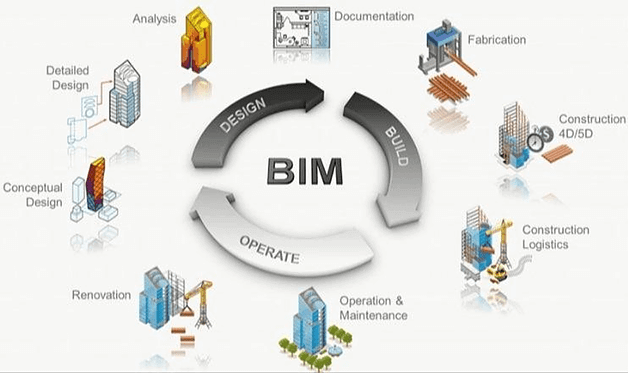
\includegraphics[scale=0.5]
    {Imagens/3.1.1-bim.png} 
    \end{center} 
    \caption{\label{img:3.1.1} Representação do BIM - Fonte: \citeauthor{hoch}} 
\end{figure}

%%%%%%%%%%%%%%%%%%%%%%%%%%%%%%%%%%%%%%%%%%%%%%%%%%%%%%%%%%%%%%%%%%%%%%%%%%%%%%%%%%%%%%%%%%%%%%
\section {Aprendizado de Máquina}

O Aprendizado de Máquina (AM) é um ramo da Inteligência Artificial (IA) que permite aos computadores aprenderem comportamentos, identificarem padrões e tomarem decisões com interação mínima de seres humanos \cite{mitchell1997}. A partir de um conjunto de dados, os algoritmos passam por um processo de treinamento, gerando um modelo que possa lidar com novas situações e resolver problemas \cite{tan2006}.

Existem três principais tipos de aprendizagem:

\begin{itemize}
    \item \textbf{Aprendizagem supervisionada}: ocorre quando um conjunto de dados previamente rotulados é utilizado para treinar o modelo, permitindo que ele preveja rótulos desconhecidos. Esse tipo de aprendizagem é capaz de tomar decisões precisas quando novos dados rotulados são fornecidos. Para estimar rótulos, isso pode ser feito por meio de dois tipos principais de tarefa: classificação e regressão. A classificação é utilizada para categorizar os dados em classes específicas, enquanto a regressão busca prever valores contínuos baseados em dados históricos \cite{faceli2011}.

    \item \textbf{Aprendizagem não supervisionada}: ocorre quando um conjunto de dados não possui nenhum rótulo associado. Nesse contexto, o objetivo é identificar padrões ou similaridades entre os dados analisados. Essa forma de aprendizagem é amplamente aplicada em problemas de agrupamento, recomendações e detecção de anomalias. Nesse caso, mesmo que os dados não sejam rotulados, eles podem ser classificados como similares ou agrupados com base nos padrões identificados \cite{faceli2011}.

    \item \textbf{Aprendizagem por reforço}: consiste em um processo de tentativa e erro, onde a máquina aprende quais ações resultam em maiores recompensas. A cada decisão tomada, o agente recebe uma recompensa ou uma punição, e o objetivo é maximizar as recompensas ao longo do tempo. Essa abordagem é amplamente utilizada em jogos e aplicações onde a máquina precisa tomar decisões sequenciais, como, por exemplo, em sistemas de controle ou simulações em ambientes complexos \cite{cerri2017}.
\end{itemize}

Nos problemas de classificação, o algoritmo busca criar um modelo capaz de generalizar os padrões extraídos do conjunto de treinamento para categorizar novas instâncias de dados não vistos. Já nos problemas de regressão, o objetivo do algoritmo é estimar valores contínuos, como, por exemplo, prever as vendas futuras de um produto ou estimar o preço de um imóvel com base em características históricas \cite{guimaraes2019}.

Um exemplo de problema de classificação é o mapeamento de uma imagem para classificar um indivíduo como homem ou mulher, ou a utilização de um classificador de sentimentos, onde o modelo pode determinar se um texto é positivo ou negativo. Por outro lado, exemplos de problemas de regressão incluem algoritmos que preveem vendas de produtos, estimam o valor de um imóvel ou calculam a expectativa de vida de um país.

Esse processo de aprendizagem é estruturado em etapas conhecidas como Fluxo de Aprendizagem de Máquina, que incluem: obtenção dos dados; preparação, limpeza e manipulação dos dados; escolha e treinamento do modelo; teste dos dados; avaliação do modelo; e melhorias do modelo \cite{tan2006}. A qualidade dos dados desempenha um papel fundamental no AM, pois o conhecimento extraído é diretamente influenciado pela qualidade das informações fornecidas \cite{guimaraes2019}. Portanto, é necessário um processo rigoroso de pré-processamento dos dados antes da aplicação dos algoritmos de AM.

O pré-processamento de dados é essencial, especialmente devido à presença de ruídos nos dados. Essa etapa pode incluir a detecção e remoção de anomalias, o tratamento de valores ausentes ou até mesmo a exclusão de atributos irrelevantes. Todo esse esforço visa aumentar a qualidade do treinamento do modelo. O sucesso do pré-processamento depende diretamente da habilidade do profissional em identificar problemas nos dados e utilizar métodos adequados para solucioná-los \cite{neves2003}.

Além das dificuldades no pré-processamento, também podem surgir problemas nas fases de treinamento e teste. Um dos desafios mais comuns é o overfitting, que ocorre quando o modelo se ajusta excessivamente aos dados de treinamento, tornando-se incapaz de generalizar para novos dados. Outro problema é o underfitting, quando o modelo não consegue capturar padrões suficientes nos dados, resultando em um desempenho insatisfatório \cite{russel2010}.

Uma vez que o modelo é construído, torna-se essencial medir seu desempenho. Entre as métricas mais comuns utilizadas para esse propósito estão:

\begin{itemize} 
    \item A \textbf{acurácia (ACC ou \textit{accuracy})}: É uma métrica muito utilizada na literatura, e sua fórmula calcula o número de acertos dividido pelo número total (número de acertos + número de erros). Essas informações são retiradas da matriz de confusão (Equação \ref{eq:3.3.1}). A matriz de confusão (Figura \ref{img:3.3.1}) é uma tabela que mostra o desempenho de um algoritmo de classificação. Se o problema de classificação for binário, ela apresentará quatro informações, que são:
    
    \begin{equation}
        ACC = \frac {(TP + TN)} {(TP + FN + FP + TN)}
        \label{eq:3.3.1}
    \end{equation}

   \begin{itemize}
        \item \textbf{Verdadeiro Positivo (TP ou \textit{True Positive})}: Ocorre quando a classe que estamos buscando foi prevista corretamente. Exemplo: a pessoa está doente, e o modelo previu corretamente que está doente;
        
        \item \textbf{Falso Positivo (FP ou \textit{False Positive})}: Ocorre quando a classe que estamos buscando foi prevista incorretamente. Exemplo: a pessoa não está doente, mas o modelo previu incorretamente que está doente;
        
        \item \textbf{Verdadeiro Negativo (TN ou \textit{True Negative})}: Ocorre quando a classe que não estamos buscando prever foi prevista corretamente. Exemplo: a pessoa não está doente, e o modelo previu corretamente que não está doente;
        
        \item \textbf{Falso Negativo (FN ou \textit{False Negative})}: Ocorre quando a classe que estamos buscando foi prevista incorretamente. Exemplo: a pessoa está doente, mas o modelo previu incorretamente que não está doente.
        \end{itemize}

        \begin{figure}[htb]
            \centering
            \caption{Matriz de confusão.}
        	\begin{center}
                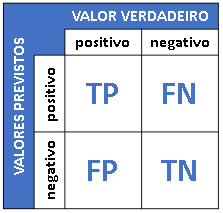
\includegraphics[scale=1]{Imagens/3.3.1-matrizconfusao.png}
        	\end{center}
            \label{img:3.3.1}
        	Fonte: Própria (2024).
        \end{figure}

    \item A \textbf{precisão (PRE ou \textit{precision})}: É utilizada para trabalhar somente com os valores positivos, e sua fórmula é calculada pelos valores verdadeiros positivos divididos pelo total de predições positivas (verdadeiro positivo + falso positivo) (Equação \ref{eq:3.3.2}).
    
    \begin{equation}
        PRE = \frac {TP} {(TP + FP)}
        \label{eq:3.3.2}
    \end{equation}

    \item A \textbf{revocação (REC ou \textit{recall})}: É utilizada para encontrar exemplos de uma classe, e sua fórmula é calculada pelos valores verdadeiros positivos divididos pelo número de resultados que deveriam ser apresentados (verdadeiro positivo + falso negativo) (Equação \ref{eq:3.3.3}).
    
    \begin{equation}
        REC = \frac {TP} {(TP + FN)}
        \label{eq:3.3.3}
    \end{equation}

    \item A \textbf{medida F1 (F1S ou \textit{F1-Score})}: É a junção da precisão com a revocação, resultando em um número único que indica a qualidade geral do modelo (Equação \ref{eq:3.3.4}). O cálculo da medida F1 é dado por:
    
    \begin{equation}
        F1S = \frac {2 \cdot PRE \cdot REC} {PRE + REC}
        \label{eq:3.3.4}
    \end{equation}
\end{itemize}

Outro conceito relevante no contexto de AM é a transferência de aprendizado (Transfer Learning), que envolve a reutilização de modelos treinados para resolver problemas relacionados em outros domínios. Essa abordagem busca aproveitar o conhecimento adquirido em uma tarefa para facilitar o aprendizado em outra tarefa, mesmo que os conjuntos de dados sejam diferentes \cite{shao2015}.

Finalmente, o Aprendizado Profundo (\textit{Deep Learning}) é uma técnica avançada de AM que utiliza redes neurais profundas, inspiradas nos neurônios do cérebro humano. Essas redes são compostas por camadas de entrada, ocultas e saída, e transformam dados em informações úteis por meio de processos sequenciais. O aprendizado profundo é amplamente utilizado em aplicações como reconhecimento de imagens, processamento de linguagem natural e sistemas de recomendação \cite{arroyo2000}


%%%%%%%%%%%%%%%%%%%%%%%%%%%%%%%%%%%%%%%%%%%%%%%%%%%%%%%%%%%%%%%%%%%%%%%%%%%%%%%%%%%%%%%%%%%%%%
\section {PLN}

Na década de 1950, Alan Turing (conhecido como o pai da computação) propôs o Teste de Turing, um experimento no qual um sistema tenta determinar se está interagindo com um ser humano ou uma máquina. Esse teste marcou o início das reflexões sobre o Processamento de Linguagem Natural (PLN) \cite{russel2010}.

O Processamento de Linguagem Natural (PLN) tem como objetivo permitir que computadores realizem tarefas relacionadas à linguagem humana, criando uma interação entre máquinas e humanos por meio de linguagem falada e/ou escrita \cite{jurafsky2009}. Segundo Liddy, o PLN é uma técnica que analisa e representa textos de maneira natural, buscando alcançar um processamento de linguagem semelhante ao do ser humano em diversas aplicações \cite{liddy1998}.

Entretanto, as linguagens naturais, como o Português e o Inglês, não possuem regras determinísticas e apresentam ambiguidades. Isso as diferencia das linguagens formais, como Python ou Java, que possuem conjuntos de regras bem definidos. Nas linguagens formais, frases precisam seguir a gramática para serem válidas, e sua semântica é projetada para evitar ambiguidades.

Os sistemas de PLN podem ser classificados de acordo com o nível de unidade linguística processada \cite{liddy1998}, como segue:

\begin{itemize}
    \item \textbf{Nível Fonológico}: Interpretação dos sons da língua. Um exemplo é a diferenciação entre as palavras "faca" e "vaca" por meio do som.
    \item \textbf{Nível Morfológico}: Análise da função, estrutura e flexão das palavras. Por exemplo, identificar que "andar" é um verbo que indica ação.
    \item \textbf{Nível Lexical}: Análise do significado das palavras, incluindo suas relações semânticas. Por exemplo, compreender que "pedra" está associada a palavras como "pedregulho", "pedraria" e "pedrinha".
    \item \textbf{Nível Sintático}: Estudo da estrutura das frases e de como são organizadas para transmitir significado.
    \item \textbf{Nível Semântico}: Análise do significado das palavras e frases, como identificar que o verbo "levar" pode significar transportar, carregar ou guiar, dependendo do contexto.
    \item \textbf{Nível de Discurso}: Interpretação de textos mais extensos, considerando sua estrutura e significado.
    \item \textbf{Nível Pragmático}: Compreensão do contexto comunicacional. Por exemplo, quando alguém diz "Nossa, as janelas estão todas abertas! Como está frio aqui!" e outra pessoa responde "Vou fechá-las", é possível inferir a intenção implícita da primeira pessoa.
\end{itemize}

De acordo com Bulengo, o PLN pode ser dividido em quatro etapas principais: análise morfológica, análise sintática, análise semântica e análise pragmática, que são executadas nessa ordem \cite{bulegon2010}. Santos, no entanto, afirma que geralmente são utilizadas apenas as três primeiras análises. Na análise morfológica, por exemplo, identificam-se substantivos, verbos e adjetivos, gerando um "dicionário" que é usado na análise sintática para compreender as relações entre palavras, como sujeito, predicado e complementos. Por fim, a análise semântica examina os termos ambíguos e seus significados no contexto \cite{santos2015}.

Na prática, raramente todos os níveis são implementados em um sistema, devido à complexidade crescente à medida que se avança nos níveis. No entanto, o PLN tem ampla aplicação, como em reconhecedores e sintetizadores de fala, corretores ortográficos, tradutores automáticos, sistemas de geração e resumo de texto, extração de informações e interfaces de linguagem natural \cite{vieira2001}.

Com o crescimento do PLN, pesquisadores têm buscado fundamentação em diversas áreas, como Filosofia da Linguagem, Psicologia, Matemática, Linguística e Ciência da Computação. Assim como no Aprendizado de Máquina (AM), o PLN exige etapas de pré-processamento que estruturam a linguagem, reduzindo o vocabulário e melhorando o desempenho dos modelos \cite{rezende2011}.

Entre as principais tarefas de pré-processamento no PLN, destacam-se:

\begin{itemize}
    \item \textbf{Normalização}: Remoção de caracteres especiais, tags HTML/CSS, e transformação de letras maiúsculas em minúsculas.
    \item \textbf{Tokenização}: Separação do texto em unidades mínimas chamadas "tokens", que podem ser palavras, símbolos ou caracteres.
    \item \textbf{Stemização}: Redução das palavras ao seu radical, como transformar "meninas" em "menin".
    \item \textbf{Lematização}: Redução das palavras à sua forma base ou lema, como transformar "meninas" e "meninos" em "menino".
    \item \textbf{Remoção de Stopwords}: Exclusão de palavras frequentes e pouco informativas, como "a", "de", "e".
    \item \textbf{Correção Ortográfica}: Tratamento de erros de digitação e abreviações para evitar problemas nos modelos.
\end{itemize}

A representação por palavras é conhecida como vetores de palavras (ou \textit{word embeddings}), onde a ideia é transformar as palavras em números, mantendo suas relações com outras palavras. Esse processo se baseia em um \textit{corpus} (um conjunto de textos a partir do qual as relações serão aprendidas). A primeira etapa é dividir o texto em palavras; em seguida, cada uma delas é representada por vetores, onde o tamanho do vetor corresponde ao número de dimensões definidas pelo \textit{corpus}. A Figura \ref{img:3.5.3} ilustra o \textit{word embeddings} com 3 dimensões (morfológica, tamanho e cor), representando um conceito completo.

    \begin{figure}[htb]
        \centering
        \caption{Exemplo da transformação de palavras em \textit{word embeddings}.}
    	\begin{center}
            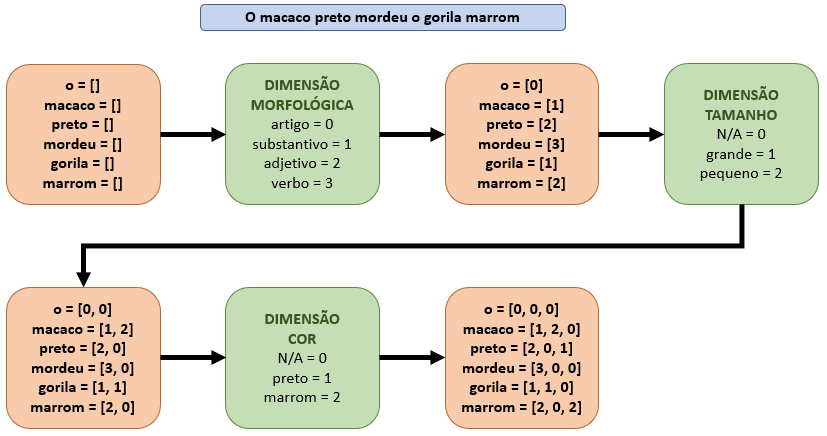
\includegraphics[scale=0.6]
            {Imagens/3.5.3-wordembeddings.png}
    	\end{center}
        \label{img:3.5.3}
    	Fonte: Própria (2021).
    \end{figure}

As vantagens do \textit{word embeddings} incluem:

\begin{itemize}
    \item \textbf{Representação Sem Contexto}: As palavras são analisadas independentemente do contexto imediato, o que pode limitar certas nuances, mas ainda permite categorizações úteis.
    \item \textbf{Relações Semânticas}: Em um espaço n-dimensional, palavras com significados similares estão próximas umas das outras, como "macaco" e "gorila".
    \item \textbf{Operações Matemáticas}: É possível realizar operações vetoriais para descobrir relações semânticas entre palavras. Por exemplo, somar um vetor associado a uma característica específica a outro vetor pode resultar em uma nova palavra relacionada.
\end{itemize}

Enquanto no exemplo acima a intuição foi usada para criar as dimensões, na Inteligência Artificial modelos baseados em Aprendizado Profundo são comumente aplicados. Eles classificam palavras em dimensões com base no contexto em que aparecem. Quanto maior o \textit{corpus}, mais precisas e eficientes tendem a ser essas representações \cite{bengio2003}.

Além do conceito de \textit{word embeddings}, existe o \textit{sentence embeddings}, que considera não apenas as palavras, mas também a ordem em que aparecem na frase \cite{conneau2017}. No \textit{sentence embeddings}, cada palavra é representada por seu \textit{word embedding}, e o conjunto dessas palavras forma uma frase completa, com informações semânticas representadas por vetores, facilitando a compreensão do contexto e da intenção da frase (Figura \ref{img:3.5.4}).

    \begin{figure}[htb]
        \centering
        \caption{Exemplo da transformação de \textit{word embeddings} para \textit{sentence embeddings}.}
    	\begin{center}
            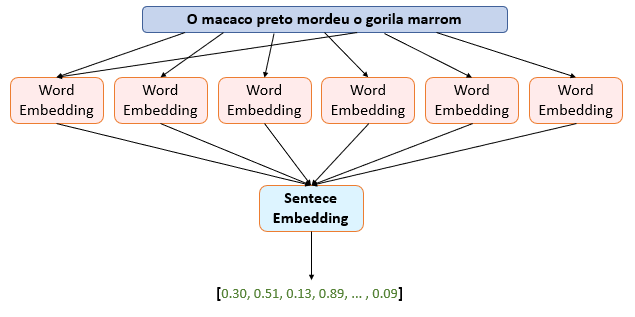
\includegraphics[scale=0.9]
            {Imagens/3.5.4-sentenceembeddings.png}
    	\end{center}
        \label{img:3.5.4}
    	Fonte: Própria (2021).
    \end{figure}

Diversas técnicas foram desenvolvidas para representar palavras vetorialmente (\textit{word embeddings}), diferenciando-se por suas arquiteturas e bases de dados usadas no treinamento \cite{martin2009}. Além disso, essas técnicas podem ser transferidas para domínios semelhantes em um processo chamado Transferência de Aprendizado, que será discutido em outra seção.

No contexto do PLN moderno, representações vetoriais, como \textit{word embeddings} e \textit{sentence embeddings}, têm sido amplamente utilizadas. Modelos como Word2Vec, GloVe, fastText e OpenAIEmbeddings destacam-se no campo \cite{devlin2019}. O OpenAIEmbeddings, em particular, apresenta um desempenho robusto em diversas tarefas de PLN.

%%%%%%%%%%%%%%%%%%%%%%%%%%%%%%%%%%%%%%%%%%%%%%%%%%%%%%%%%%%%%%%%%%%%%%%%%%%%%%%%%%%%%%%%%%%%%%
\section {Redes Neurais Artificiais}

O sistema nervoso humano é composto por neurônios, que desempenham a função de transmitir informações essenciais para o funcionamento, comportamento e raciocínio do corpo humano \cite{tafner1995}. As Redes Neurais Artificiais (RNAs) são técnicas computacionais inspiradas na estrutura neural do ser humano, adquirindo conhecimento por meio da experiência \cite{haykin1999}. Assim, uma rede neural artificial pode ser compreendida como uma abstração da rede neural biológica, com o objetivo de modelar processos de aprendizado e resolver problemas complexos.

O primeiro modelo que simulou uma rede neural biológica foi desenvolvido em 1943 pelos psiquiatras Warren McCulloch e Walter Pitts. Esse trabalho apresentou detalhes sobre o comportamento e a memória dos neurônios biológicos em uma forma artificial, mas não abordou como o aprendizado poderia ser implementado \cite{mcculloch1943}). Já em 1949, Donald Hebb conduziu o primeiro estudo voltado à fase de aprendizado das redes neurais artificiais, demonstrando que os pesos em cada conexão entre neurônios resultavam em uma força de excitação, similar à encontrada nos neurônios biológicos \cite{hebb1949}. Entretanto, esse modelo ainda não possuía a capacidade de reconhecer padrões.

Em 1958, Rosenblatt desenvolveu o primeiro modelo capaz de detectar padrões e características, demonstrando que, ao modificar os pesos conectados aos neurônios, o modelo poderia ser treinado para classificar padrões \cite{rosenblatt1958}. Este modelo ficou conhecido como perceptron e apresenta uma arquitetura composta por três camadas:

\begin{itemize}  
    \item \textbf{Camada de entrada}: Responsável por receber informações do ambiente externo e repassá-las às camadas intermediárias.
    \item \textbf{Camadas intermediárias (ou ocultas)}: Processam os sinais recebidos, ajustam os pesos e enviam as informações para a camada seguinte.
    \item \textbf{Camada de saída}: Produz e apresenta o resultado final.
\end{itemize}

Contudo, quando utilizado para classificar padrões, uma rede perceptron de três camadas é limitada a encontrar uma única solução. Para resolver problemas que exigem múltiplas soluções, Minsky e Papert propuseram a inclusão de múltiplas camadas intermediárias, resultando no modelo conhecido como perceptron multicamadas (\textit{Multi-layer Perceptron} – MLP) \cite{minsky1969}.

O MLP é composto por um conjunto de neurônios conectados em paralelo, com cada conexão associada a um peso que reflete sua influência na rede. A partir da interação em camadas intermediárias, onde a saída de um neurônio se torna a entrada de outro, obtém-se um comportamento inteligente, capaz de reconhecer padrões e características \cite{soares2015}.

A estrutura de um neurônio em uma rede MLP processa informações recebidas do ambiente externo (valores x) associadas a pesos (w). Uma soma ponderada dos produtos de x e w é então calculada, somando-se o limiar de ativação (bias ou polarização). O valor resultante, chamado de ponto de ativação (u), é avaliado por uma função de ativação que limita a amplitude da saída do neurônio, geralmente dentro do intervalo [0, 1], podendo ser interpretado como uma probabilidade \cite{goodfellow2016}.

\begin{figure}[htb]
    \centering
    \caption{Rede Neural MLP.}
    \begin{center}
        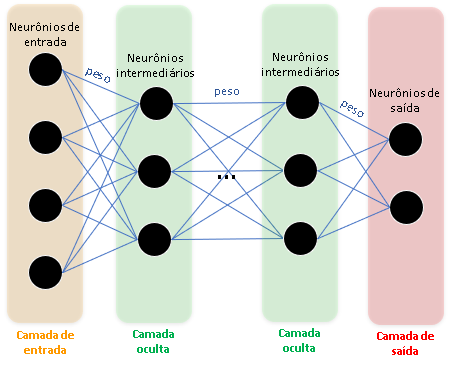
\includegraphics[scale=1]
        {Imagens/3.4.1-rna.png}
    \end{center}
    \label{img:3.2.1}
    Fonte: Própria (2024).
\end{figure}

A Figura \ref{img:3.4.2} demonstra o processamento de informações por um neurônio em uma rede MLP, onde, dado um conjunto de valores '\textit{x}' (que representam as informações do mundo externo), esses valores são associados a pesos '\textit{w}'. A partir disso, é efetuada uma soma ponderada dos produtos '\textit{x}' e '\textit{w}', à qual é somado o limiar de ativação (bias ou polarização), como mostrado na Equação \ref{eq:3.4.1}.

\begin{figure}[htb]
    \centering
    \caption{Estrutura de um neurônio no MLP.}
    \begin{center}
        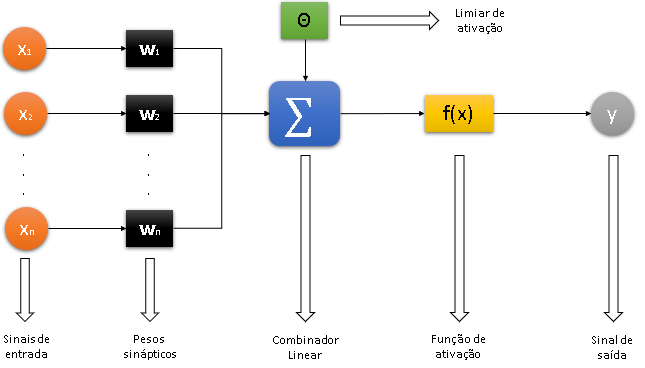
\includegraphics[scale=0.9]
        {Imagens/3.4.2-rnamlp.png}
    \end{center}
    \label{img:3.4.2}
    Fonte: Própria (2024).
\end{figure}

\begin{equation}
    u = \sum_{i=1}^{n} x_{i} \cdot w_{i} + \theta
    \label{eq:3.4.1}
\end{equation}

O bias ($\theta$) é responsável pelo deslocamento inicial da função de ativação no plano onde ela é representada. Caso o bias seja positivo, o movimento é realizado para a esquerda, diminuindo o valor do eixo x. Caso seja negativo, o movimento é realizado para a direita, aumentando o valor do eixo x \cite{rojas1996}, como ilustrado na Figura \ref{img:3.4.3}.

\begin{figure}[htb]
    \centering
    \caption{Exemplo do deslocamento do gráfico através da mudança da constante bias.}
    \begin{center}
        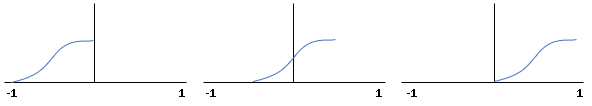
\includegraphics[scale=1]
        {Imagens/3.4.3-bias.png}
    \end{center}
    \label{img:3.4.3}
    Fonte: Própria (2024).
\end{figure}

O valor \textit{u} obtido, chamado de ponto de ativação, é avaliado pela função de ativação, que é responsável por calcular o sinal da saída do neurônio. A função de ativação, também conhecida como função de transferência, tem o objetivo de limitar a amplitude da saída do neurônio. Ou seja, o valor obtido estará no intervalo entre 0 e 1, podendo ser interpretado como uma probabilidade do resultado \cite{goodfellow2016}.

Existem diversos tipos de funções de ativação, e não há uma regra fixa para determinar qual é melhor ou pior. A escolha depende do problema, embora, dependendo das propriedades específicas, seja possível optar por uma função que facilite e acelere a convergência da rede neural \cite{goodfellow2016}.

As funções de ativação mais populares são:

\begin{itemize}
    \item \textbf{Função de Etapa Binária} ($ f(x) = 1$, se x>=0 e $f(x) = 0$, se x<0): Essa função determina se o neurônio deve ou não estar ativo. Caso o valor '\textit{u}' seja maior que um limite pré-determinado, o neurônio é ativado; caso contrário, ele permanece desativado. Embora útil em classificadores binários, é mais utilizada como referência teórica, pois, no processo de retropropagação (backpropagation), os gradientes das funções de ativação retornam zero, o que impede a melhoria dos resultados \cite{feng2019}.

    \item \textbf{Função Linear} ($ f(x) = ax $): Nessa função, cada camada passa por uma transformação linear. No entanto, essa função possui limitações semelhantes à função de etapa binária, já que sua derivada é constante, independentemente do valor da entrada. Isso impede melhorias durante o backpropagation \cite{feng2019}.

    \item \textbf{Função Sigmoid} ($ f (x) = 1 / (1 + e^{-x}) $): Essa função comprime os valores de saída para o intervalo entre 0 e 1, o que é útil para classificar uma classe específica. Embora não seja linear e permita saídas não lineares em redes neurais, apresenta dois problemas principais: 1) os gradientes podem se aproximar de zero, o que prejudica o aprendizado da rede, e 2) os valores de saída são sempre positivos, o que pode não ser desejável em todos os casos. Apesar disso, ela é amplamente utilizada em classificadores \cite{feng2019}.

    \item \textbf{Função Tanh} ($f (x) = 2 / (1 + e ^{(-2x)}) -1$): É uma variação escalonada da função Sigmoid, mas simétrica em relação à origem, variando de -1 a 1. Isso elimina o problema dos valores positivos constantes. As demais propriedades são semelhantes às da Sigmoid \cite{feng2019}.

    \item \textbf{Função ReLU} ($ f(x) = max(0,x) $): É a função de ativação mais amplamente utilizada no design de redes neurais. Por ser não linear, facilita a propagação dos erros e melhorias durante o treinamento. Sua principal vantagem é não ativar todos os neurônios simultaneamente, tornando a rede mais eficiente. No entanto, pode sofrer com o problema de gradientes que convergem para zero \cite{feng2019}.

    \item \textbf{Função Leaky ReLU} ($f(x) = ax$, se x < 0 e $f(x) = x$, se x >= 0): Uma variação da ReLU que corrige o problema do gradiente zero. Quando '\textit{x}' < 0, é aplicada uma componente linear em vez de zero, garantindo um gradiente constante mesmo para valores negativos. É especialmente útil em camadas ocultas e para lidar com neurônios defeituosos \cite{feng2019}.

    \item \textbf{Função Softmax}: É uma extensão da Sigmoid, projetada para problemas de classificação com múltiplas classes. Transforma as saídas de cada classe em valores entre 0 e 1, normalizando-as para que sua soma seja igual a 1. Assim, é possível interpretar os resultados como probabilidades de pertencimento a cada classe \cite{sensoy2018}.
\end{itemize}

O treinamento de uma rede neural artificial multicamadas consiste em ajustar os pesos sinápticos e o bias de modo que as saídas se aproximem das saídas esperadas. Esse processo ocorre em duas etapas \cite{russel2010}:

\begin{itemize}
    \item \textbf{Propagação (forward-propagation)}: Nesta etapa, aplica-se a Equação 3.7 em cada neurônio. O fluxo de dados começa na camada de entrada, atravessa as camadas ocultas e finaliza na camada de saída \cite{hafemann2014}.
    
    \item \textbf{Retropropagação (backpropagation)}: Após a etapa de propagação, os valores de saída são comparados com os valores desejados usando uma função custo, que mede o desempenho da rede. Caso o desempenho seja insatisfatório, inicia-se a retropropagação para minimizar o erro, ajustando os pesos e os bias. Isso é feito utilizando o método do Gradiente Descendente \cite{hafemann2014}.
    
    \begin{itemize}
        \item \textbf{Função Custo (Loss)}: Mede o quão distante está a saída da rede em relação à saída esperada. Para regressão, a função mais comum é o Erro Quadrático Médio (MSE). Para classificação, é a Entropia Cruzada \cite{mccaffrey2013}.
        
        \item \textbf{Erro Quadrático Médio (MSE)}: Mede a diferença entre os valores previstos e os reais, elevando ao quadrado e calculando a média (Equação \ref{eq:3.4.5}) \cite{willmott1981}.

            \begin{equation}
                MSE = \frac{1}{n} \sum_{i=1}^{n} (\theta_{ip} - \theta_{i})^2 
                \label{eq:3.4.5}
            \end{equation}
        
        \item \textbf{Raiz do Erro Quadrático Médio (RMSE)}: Similar ao MSE, mas calcula a raiz quadrada da média dos erros (Equação \ref{eq:3.4.2}) \cite{chai2014}.

            \begin{equation}
                RMSE = \sqrt{\frac{1}{n} \sum_{i=1}^{n} e_i^2}
                \label{eq:3.4.2}
            \end{equation}
        
        \item \textbf{Erro Médio Absoluto (MAE)}: Mede o desvio médio entre valores previstos e reais, com pesos iguais para todos os desvios (Equação \ref{eq:3.4.6}) \cite{willmott1981}.

            \begin{equation}
                MAE = \frac{ \sum_{i=1}^{n} |O_{i} - P_{i}|}{n}
                \label{eq:3.4.6}
            \end{equation}
        
        \item \textbf{Entropia Cruzada}: Mede a distância entre os vetores de saída e os valores esperados (Equação \ref{eq:3.4.3}) \cite{nasr2002}.

            \begin{equation}
                E(w) = \frac{1}{n} \cdot \sum_{i=1}^{n} [t_{i} \cdot log(y_{i}) + (1 - t_{i}) \cdot log(1 - y_{i})]
                \label{eq:3.4.3}
            \end{equation}
        
        \item \textbf{Gradiente Descendente}: Método de otimização que ajusta pesos e bias na direção que minimiza o erro. A cada iteração, busca-se o mínimo local da função custo (Equação \ref{eq:3.4.4}) \cite{rumelhart1986}.

            \begin{equation}
                (\mathbf{w},b) \leftarrow (\mathbf{w},b) - \frac{\eta}{|\mathcal{B}|} \sum_{i \in \mathcal{B}} \partial_{(\mathbf{w},b)} l^{(i)}(\mathbf{w},b)
                \label{eq:3.4.4}
            \end{equation}
    \end{itemize}
\end{itemize}

Cada ciclo de propagação e retropropagação ajusta os pesos para reduzir a função de perda, repetindo o processo até atingir o erro mínimo local \cite{russel2010}.

Um dos ramos do Aprendizado de Máquina baseado em Redes Neurais Artificiais é o Aprendizado Profundo (ou Deep Learning), que utiliza diversas camadas capazes de extrair características em diferentes níveis. Por exemplo, em um processamento de imagem, a primeira camada pode extrair formas gerais, como objetos ou rostos humanos, enquanto camadas posteriores extraem características mais específicas, como bordas e cantos. Ou seja, as camadas iniciais extraem recursos de baixo nível, enquanto as camadas mais profundas extraem recursos de alto nível e/ou médio nível \cite{schmidhuber2015}.

Um dos principais benefícios da Aprendizagem Profunda é sua capacidade de extrair características automaticamente, utilizando pesos adaptáveis no kernel, o que economiza tempo ao evitar a necessidade de pré-processamento manual \cite{schmidhuber2015}. Nesse contexto, uma rede neural artificial possui três tipos de camadas, e os nós (ou nodos) podem ter dois tipos de conexões, que são:

\begin{itemize}
    \item \textbf{Redes de camada única}: ocorre quando há apenas um nó entre qualquer entrada e saída da rede (Figura \ref{img:3.4.4} (a) e (c)) \cite{braga2000}.
    \item \textbf{Redes de múltiplas camadas}: ocorre quando há mais de um neurônio entre qualquer entrada e saída da rede (Figura \ref{img:3.4.4} (b) e (d)) \cite{braga2000}.
    \item \textbf{Redes recorrentes}: ocorre quando existe pelo menos um laço de realimentação em alguma camada (Figura \ref{img:3.4.4} (c) e (d)) \cite{braga2000}.
    \item \textbf{Nó acíclico (feedforward)}: ocorre quando a saída de um neurônio não é utilizada como entrada em camadas anteriores ou iguais (Figura \ref{img:3.4.4} (a) e (b)) \cite{haykin2001}.
    \item \textbf{Nó cíclico (feedback)}: ocorre quando a saída de um neurônio é utilizada como entrada em camadas anteriores ou iguais (Figura \ref{img:3.4.4} (c) e (d)) \cite{haykin2001}.
\end{itemize}

\begin{figure}[htb]
        \centering
        \caption{Tipos de camadas e conexões de nodos.}
    	\begin{center}
            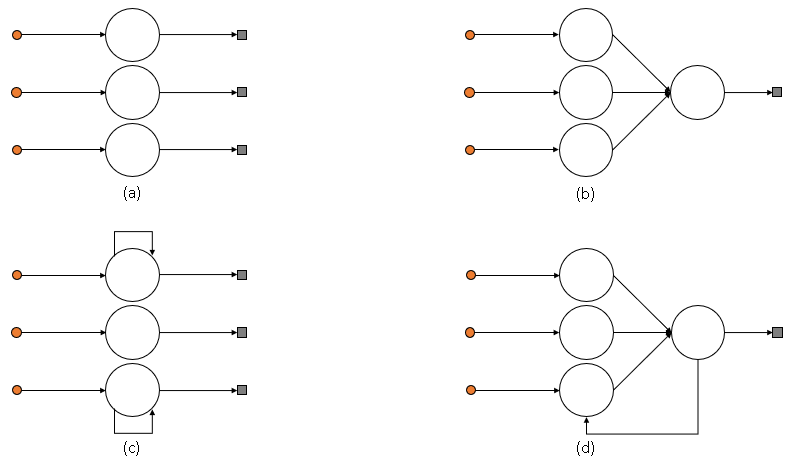
\includegraphics[scale=0.6]
            {Imagens/3.4.4-tiposrna.png}
    	\end{center}
        \label{img:3.4.4}
    	Fonte: Própria (2024).
    \end{figure}

Ou seja, Redes Neurais Recorrentes (Recurrent Neural Networks ou RNN) diferem substancialmente das tradicionais Redes Neurais Feedforward (FNN), pois possuem ciclos, permitindo que os dados de saída sejam alimentados de volta nas camadas anteriores. Isso torna o modelo capaz de capturar dependências temporais entre os dados \cite{ramakrishnan2018}.

O ciclo presente nas RNNs permite que essas redes utilizem seu estado interno (memória) para processar entradas sequenciais, o que é essencial para tarefas que envolvem sequências temporais. Essa capacidade de armazenar informações passadas é especialmente útil em aplicações como reconhecimento de fala, processamento de linguagem natural, previsão de séries temporais, entre outras.

No entanto, devido à repetição de operações no ciclo das RNNs, que inclui uma matriz de pesos 
\textit{W} representando os pesos de cada neurônio em uma camada, essas redes tendem a se tornar profundas. Essa profundidade pode gerar problemas como a dissipação do gradiente (gradient vanishing) e a explosão do gradiente (gradient explosion) \cite{goodfellow2016}.

A dissipação do gradiente ocorre quando os erros das últimas camadas afetam pouco os erros nas camadas iniciais, prejudicando o treinamento da rede. Isso acontece porque, durante as atualizações, os pesos e o bias das camadas iniciais não são significativamente ajustados. Por outro lado, a explosão do gradiente faz com que os gradientes nas camadas iniciais fiquem muito grandes, tornando a rede instável \cite{goodfellow2016}.

Para mitigar esses problemas, os cientistas Hochreiter e Schmidhuber propuseram o LSTM (\textit{Long Short-Term Memory} ou Memória de Longo e Curto Prazo). Nesse modelo, os neurônios tradicionais foram substituídos por células de memória, permitindo que as redes RNN superem as limitações associadas à dissipação e à explosão do gradiente \cite{hochreiter1997}.

%%%%%%%%%%%%%%%%%%%%%%%%%%%%%%%%%%%%%%%%%%%%%%%%%%%%%%%%%%%%%%%%%%%%%%%%%%%%%%%%%%%%%%%%%%%%%%
\section {Memória Longa de Curto Prazo}

O LSTM é uma evolução do RNN. O funcionamento dessa rede é estruturado de forma em cadeia, onde cada camada representa um intervalo de tempo \textit{t} e a rede possui células de memória, nas quais cada célula contém portões de entrada, de esquecimento e de saída.

\begin{itemize}
    \item \textbf{Portão de entrada (\textit{input gate})}: Tem o objetivo de atualizar, a partir do fluxo de dados de entrada, o estado de memória da célula \cite{abdelnasser2019}.
    
    \item \textbf{Portão de esquecimento (\textit{forget gate})}: Tem o objetivo de controlar qual informação deve permanecer na memória \cite{abdelnasser2019}.
    
    \item \textbf{Portão de saída (\textit{output gate})}: Tem o objetivo de determinar como a saída é influenciada pelo valor de entrada e pela memória armazenada \cite{abdelnasser2019}.
\end{itemize}

Segundo \cite{tai2015}, a primeira coisa que a célula do LSTM faz é decidir qual informação será removida ou mantida no estado atual da célula. Essa operação é realizada pelo portão do esquecimento, que retorna um valor entre 0 (esquecer) e 1 (manter). Todo esse processo é calculado pela função \textit{sigmoid} (Equação \ref{eq:3.5.1}).

\begin{equation}
    f_{t} = sigmoid(W_{f} \cdot [h_{t-1}, x_{t}] + b_{f})
    \label{eq:3.5.1}
\end{equation}
 
Em seguida, decide-se qual nova informação será armazenada. Essa decisão ocorre em duas etapas: a primeira determina qual valor deverá ser atualizado (calculada pela função \textit{sigmoid}) (Equação \ref{eq:3.5.2}), e a segunda cria um vetor de novos valores candidatos que podem ser adicionados ao estado (calculada pela função \textit{tanh}) (Equação \ref{eq:3.5.3}).

\begin{equation}
    i_{t} = sigmoid(W_{i} \cdot [h_{t-1}, x_{t}] + b_{i})
    \label{eq:3.5.2}
\end{equation}

\begin{equation}
    \tilde{C}_{t} = tanh(W_{C} \cdot [h_{t-1}, x_{t}] + b_{C})
    \label{eq:3.5.3}
\end{equation}
 
Depois disso, multiplica-se o estado antigo pelos candidatos passados ($C_{t-1}$), para esquecer as informações desnecessárias, e multiplica-se o estado atualizado pelos candidatos atuais ($\tilde{C}_{t}$), para manter as informações úteis (Equação \ref{eq:3.5.4}).

\begin{equation}
    C_{t} = f_{t} \times C_{t-1} + i_{t} \times \tilde{C}_{t}
    \label{eq:3.5.4}
\end{equation}
 
Por fim, a camada \textit{sigmoid} decide quais informações da célula irão para a saída (Equação \ref{eq:3.5.5}), e essas informações são multiplicadas pela função \textit{tanh} aplicada aos candidatos atuais, permitindo que somente as informações relevantes sejam emitidas (Equação \ref{eq:3.5.6}).

\begin{equation}
    o_{t} = sigmoid(W_{o} \cdot [h_{t-1}, x_{t}] + b_{o})
    \label{eq:3.5.5}
\end{equation}

\begin{equation}
    h_{t} = o_{t} \times tanh(C_{t})
    \label{eq:3.5.6}
\end{equation}

A LSTM possui uma estrutura computacional complexa que opera com base na ativação de diferentes funções, decidindo quais informações devem ser mantidas, alteradas ou descartadas. Essa rede tem alcançado grande sucesso na solução de tarefas sequenciais \cite{tai2015}. Com esse sucesso, surgiu uma variante denominada \textit{Bidirectional Long Short-Term Memory} (BiLSTM ou Memória Longa de Curto Prazo Bidirecional), uma rede composta por duas LSTMs funcionando em paralelo. Uma das redes percorre a sequência para frente (\textit{Forward LSTM}), enquanto a outra percorre a sequência para trás (\textit{Backward LSTM}), permitindo capturar informações passadas e futuras, o que aumenta o poder de aprendizado da rede \cite{graves2013}.

Apesar de as redes neurais recorrentes (RNNs) apresentarem iterações eficientes, as redes \textit{Long Short-Term Memory} (LSTM), projetadas para tarefas do tipo \textit{sequence-to-sequence} (\textit{seq2seq}), recebem uma sequência de dados e produzem outra. Nesse contexto, uma estrutura neural que tem ganhado destaque no mundo do Processamento de Linguagem Natural (PLN) é o \textit{transformer}, devido ao seu desempenho em tarefas como traduções, sumarizações e legendamento de imagens, entre outras.


%%%%%%%%%%%%%%%%%%%%%%%%%%%%%%%%%%%%%%%%%%%%%%%%%%%%%%%%%%%%%%%%%%%%%%%%%%%%%%%%%%%%%%%%%%%%%%
\section {Transformers}

Redes neurais recorrentes \cite{ramakrishnan2018}, memória de curto e longo prazo \cite{hochreiter1997} e redes neurais recorrentes com portas \cite{chung2014}, em particular, foram firmemente estabelecidas como abordagens de última geração em modelagem de sequência. Redes de modelagem de sequência (\textit{seq2seq}) possuem uma abordagem na qual se utilizam modelos de Aprendizado de Máquina ou de Aprendizado Profundo para obter uma sequência de dados como entrada (em um domínio específico) e converte essa sequência para uma representação em outro domínio \cite{sutskever2014}.

Essa abordagem normalmente é realizada por meio de dois módulos: um \textit{encoder} (codificador) e um \textit{decoder} (decodificador), onde o \textit{encoder} tem o objetivo de processar a sequência de entrada e transformá-la em um contexto, enquanto o \textit{decoder} pega o contexto e produz uma sequência de saída \cite{sutskever2014}. Um exemplo de \textit{seq2seq} pode ser um modelo de tradução inglês-português, no qual o módulo \textit{encoder} transforma o texto em inglês em um "contexto livre de idioma" e, depois, o módulo \textit{decoder} adiciona a segunda língua (português) nesse contexto.

No exemplo de um modelo de tradução inglês-português, será demonstrado o \textit{encoder} e o \textit{decoder} na forma de RNNs (Redes Neurais Recorrentes), onde o \textit{encoder} processa as palavras da sequência de entrada uma a uma (de forma recorrente). A cada etapa do processamento, a palavra que entra na rede produz uma saída e um estado oculto (contexto). A saída geralmente do \textit{encoder} é descartada, enquanto o estado oculto é passado para a próxima etapa, sendo utilizado nas palavras seguintes da sequência para produzir mais uma saída e criando um novo estado oculto (ou seja, atualizando o contexto). Esse processo se repete até a última palavra da sequência de entrada, onde o \textit{encoder} cria o estado oculto final (contexto final).

Esse contexto final é passado para a segunda RNN, o \textit{decoder}, que também recebe um "vetor genérico" (os valores são ajustados durante o treinamento). Esse vetor representa o início da frase de saída e, da mesma forma que o \textit{encoder}, o \textit{decoder} utiliza o vetor e o contexto para produzir uma saída e um estado atualizado, passando por etapas (nesse exemplo, palavras), e, em cada etapa, a saída representa a palavra traduzida até chegar na última etapa (palavra), que irá entregar a frase inteira traduzida (Figura \ref{img:3.6.1}).

\begin{figure}[htb]
    \centering
    \caption{Exemplo de um modelo seq2seq para tradução do inglês para português.}
    \begin{center}
        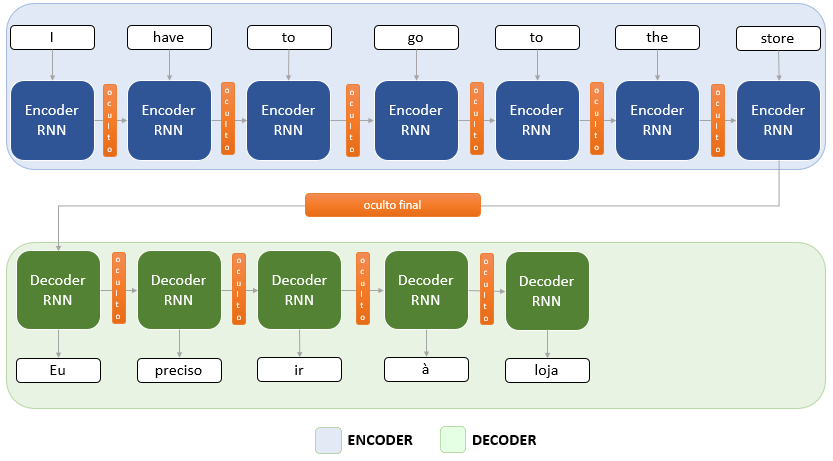
\includegraphics[scale=0.7]{Imagens/3.6.1-seq2seq.png}
    \end{center}
    \label{img:3.6.1}
    Fonte: Própria (2024).
\end{figure}

Porém, não é necessário utilizar apenas RNN para codificadores e decodificadores. É possível misturar e combinar diversos modelos, como demonstra o autor Jonghwan Mun, que utiliza um codificador CNN (\textit{Convolutional Neural Networks}) \cite{simard2003}, um codificador RNN e um decodificador LSTM para um modelo que gera legendas de imagens \cite{mun2016}.

Como pode ser visto na Figura \ref{img:3.6.1}, a frase original tem 7 palavras, enquanto a frase traduzida contém 5 palavras. Por isso, dependendo da complexidade do problema, e no caso de traduções, a tarefa de traduzir não se trata de um simples alinhamento das palavras individuais. É necessário que o modelo seja capaz de focar em uma palavra, caso seja necessário, ou em um trecho específico da frase, criando assim o conceito de atenção.

Nas RNNs, o mecanismo de atenção geralmente é implementado da seguinte forma: no \textit{encoder}, além do contexto ser representado pelo estado oculto final, ele também é representado por todos os estados ocultos produzidos após o processamento de cada palavra, fazendo com que cada estado oculto contenha o contexto acumulado até aquela palavra, o qual, após processar todas as palavras, é enviado para o \textit{decoder} juntamente com todos os estados ocultos \cite{bahdanau2015}. Ou seja, no exemplo da Figura \ref{img:3.6.1}, a palavra '\textit{go}' após ser processada, possuirá o estado oculto (contexto) acumulado das palavras '\textit{I}', '\textit{have}', '\textit{to}' e '\textit{go}'.

O \textit{decoder} recebe e extrai do estado oculto final as informações necessárias para produzir o próximo estado oculto e utiliza o acúmulo de estados ocultos anteriores para calcular uma pontuação de atenção, indicando quanto foco a etapa dará para esses contextos parciais. O resultado da pontuação de atenção é multiplicado por cada estado oculto respectivo, e depois todos são somados, gerando o resultado denominado estado de contexto (Figura \ref{img:3.6.2}). Esse estado de contexto se espera que carregue a informação de interesse de forma amplificada, ou seja, indicando qual parte da frase o modelo deve prestar mais atenção. Por fim, o estado de contexto é concatenado com o estado final produzido nesta última etapa do \textit{decoder}, onde o vetor é processado por uma estrutura de rede adicional do tipo totalmente conectada, produzindo então o vetor que representa a palavra no segundo idioma (português) \cite{bahdanau2015}.

\begin{figure}[htb]
    \centering
    \caption{Exemplo de um modelo com o mecanismo de atenção para tradução do inglês para português.}
    \begin{center}
        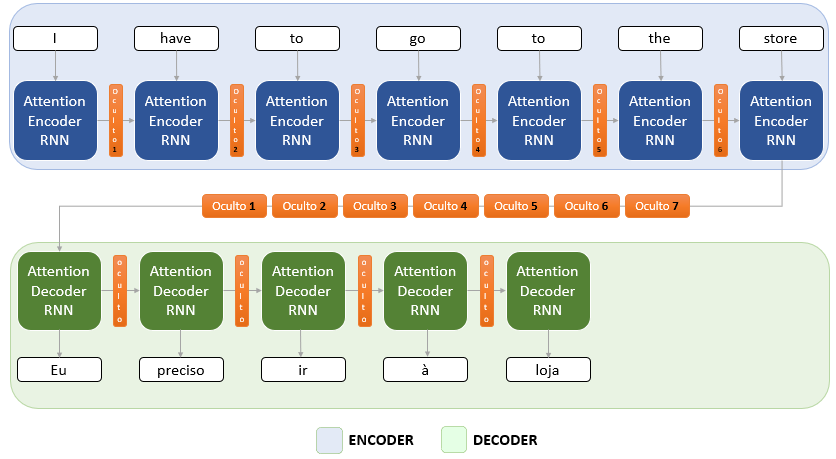
\includegraphics[scale=0.7]
        {Imagens/3.6.2-attention.png}
    \end{center}
    \label{img:3.6.2}
    Fonte: Própria (2024).
\end{figure}

De acordo com \cite{bahdanau2015}, o mecanismo de atenção obtém melhores resultados para a maioria das tarefas que necessitam "traduzir" uma sequência em outra, podendo transformar um texto em seu resumo, ou uma imagem em sua legenda. Porém, modelos recorrentes, mesmo utilizando o mecanismo de atenção (\textit{Attention}), dada a sua natureza sequencial, acabam realizando processos computacionais intensivos para captar o contexto de uma sequência. Por isso, foi criada a arquitetura \textit{transformer}, uma técnica que proporciona melhorias significativas tanto na eficiência computacional quanto na performance dos modelos baseados em arquiteturas recorrentes.

Assim como outras redes com mecanismo de atenção, o \textit{transformer} também possui os módulos \textit{encoder} e \textit{decoder}, onde os criadores do modelo criaram 6 pilhas (\textit{stacks}) de \textit{encoders} e \textit{decoders} individuais, arranjados linearmente. Cada \textit{encoder} de cada pilha possui duas unidades (camadas) chamadas de \textit{self-attention}, uma aplicando o mecanismo de atenção sobre o texto que ela recebe e outra que transforma o resultado da camada de \textit{self-attention} em um \textit{embedding} de comprimento menor \cite{vaswani2017}.

O \textit{decoder} é construído com as mesmas unidades do \textit{encoder}, porém, possui uma camada adicional denominada \textit{encoder-decoder attention}, cujo objetivo é mapear o resultado da camada de \textit{self-attention} do \textit{decoder} com os \textit{embeddings} construídos pelo \textit{encoder} \cite{vaswani2017}. Com isso, enquanto nos modelos \textit{seq2seq} as palavras são processadas sequencialmente, o \textit{transformer} recebe o texto que deve processar tudo de uma vez, onde, através de um método independente, todas as palavras são convertidas em \textit{embeddings}.

A camada \textit{self-attention} (Figura \ref{img:3.6.3}) converte cada palavra em três vetores, denominados \textit{q} (\textit{query}), \textit{k} (\textit{key}) e \textit{v} (\textit{value}), onde é feita a multiplicação dos vetores da palavra por três matrizes (pesos) $W^q$, $Q^k$ e $W^v$, respectivamente (Figura \ref{img:3.6.3} (b), (c) e (d)), cujos parâmetros são ajustados durante o treinamento da rede. Esses vetores (\textit{q}, \textit{k} e \textit{v}) são abstrações para permitir o cálculo de atenção, que é realizado por meio de uma multiplicação entre as \textit{queries} e as \textit{keys}. Essa operação irá resultar em uma pontuação que será normalizada e aplicada às \textit{values}, como mostrado na Figura \ref{img:3.6.3} (e). O resultado final de uma camada de \textit{self-attention} é uma nova sequência que leva em consideração o foco nas palavras mais importantes de toda a sequência.

\begin{figure}[htb]
    \centering
    \caption{Exemplo do cálculo de uma camada de \textit{self-attention}.}
    \begin{center}
        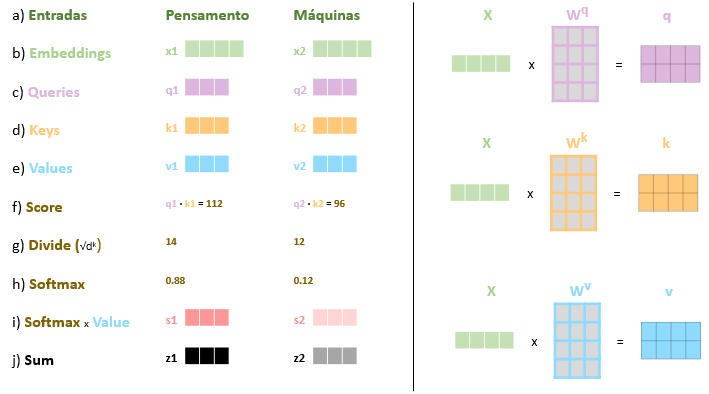
\includegraphics[scale=0.7]
        {Imagens/3.6.3-selfattention.png}
    \end{center}
    \label{img:3.6.3}
    Fonte: Própria (2024).
\end{figure}

Essa pontuação é dividida pela raiz quadrada do comprimento dos vetores \textit{k} ($\sqrt{d^k}$) para garantir maior estabilidade dos gradientes (Figura \ref{img:3.6.3} (g)). Com isso, o resultado de cada par de palavras é submetido à transformação \textit{softmax}, que gera valores no intervalo entre 0 e 1, sendo que a soma de todos os valores é igual a 1 (Figura \ref{img:3.6.3} (h)). Esse resultado representa a “atenção” que a rede deve dar a cada par de palavras. Em seguida, o valor do \textit{softmax} é multiplicado pelo vetor \textit{v} das palavras correspondentes (ou seja, a palavra com a qual a palavra-foco faz par), resultando em vetores \textit{s} (Figura \ref{img:3.6.3} (i)), que são somados, produzindo, finalmente, um vetor \textit{z} para a palavra-foco (Figura \ref{img:3.6.3} (j)), que incorpora as relações entre a palavra-foco e todas as demais palavras da sequência, com a devida atenção considerada \cite{vaswani2017}.

Todos os valores da Figura \ref{img:3.6.3} são ilustrativos; porém, os vetores \textit{s} e \textit{z} estão em diferentes tons para demonstrar que, após a multiplicação dos valores pelo \textit{softmax}, o valor de uma palavra terá maior impacto que o de outra, fazendo com que o vetor \textit{z} de uma tenha maior peso que o de seu par (neste exemplo, o $z_{1}$), demonstrando a relação entre as palavras.

O módulo \textit{encoder} possui um conjunto de matrizes $W^q$, $Q^k$ e $W^v$, e esse conjunto é denominado de \textit{attention head} (ou cabeça de atenção). A quantidade de \textit{attention heads} é a raiz quadrada do comprimento dos vetores \textit{k} ($\sqrt{d^k}$). Com isso, o \textit{transformer} realiza o mecanismo de atenção mais de uma vez, resultando, no final da camada de \textit{self-attention}, em \textit{n} ($\sqrt{d^k}$) vetores \textit{z} para cada texto, fazendo com que haja atenção em diversos dados \cite{popel2018}. Esse processo é similar ao que ocorre com o ser humano, que, por exemplo, ao ler um livro, dá atenção a diversas partes do texto ao mesmo tempo, como o nome de um personagem, o ambiente em que se situa, entre outros, e o \textit{transformer} funciona de maneira análoga.

Por fim, a última etapa é concatenar todos os vetores \textit{z} (\textit{attention heads}) e multiplicá-los por uma matriz de peso $W^o$, que também é ajustada durante o treinamento do modelo. Cada palavra será representada por um vetor \textit{z} com o mesmo tamanho do vetor \textit{v}, e esses vetores passam por uma camada \textit{feed forward}, que irá gerar os \textit{embeddings finais}, os quais são enviados pelo \textit{encoder} para o \textit{decoder}.

O \textit{decoder} recebe os \textit{embeddings} e transforma-os em matrizes de atenção \textit{K} e \textit{V}, que serão aplicadas nas camadas \textit{encoder-decoder attention}. Essa camada aplica a camada \textit{self-attention} no primeiro vetor que recebe, que, no exemplo de tradução, é o início da sequência traduzida, e esse processamento é o mesmo da camada \textit{self-attention} do \textit{encoder}. No entanto, na camada \textit{encoder-decoder attention}, são utilizadas as matrizes \textit{K} e \textit{V} (que são produtos do processamento da sequência de entrada), ao invés de utilizar as matrizes $W^k$ e $W^V$.

O resultado da pilha que forma o \textit{decoder} é, da mesma forma que no \textit{encoder}, um \textit{embedding} de comprimento igual ao \textit{embedding} que representa o texto original. Esse \textit{embedding} passa por uma camada linear, convertendo-o em um vetor que, no exemplo de tradução, tem comprimento igual ao do vocabulário do segundo idioma (português), resultando na representação de cada uma das palavras traduzidas.

Esse vetor é ativado pela função \textit{softmax}, resultando em um vetor de probabilidades, e o valor com maior probabilidade indica a palavra que o modelo deve gerar, produzindo, finalmente, uma saída (Figura \ref{img:3.6.4} (seta azul)). Ao retornar essa saída como resultado, a palavra volta para o início do \textit{decoder} (Figura \ref{img:3.6.4} (seta amarela)), para ser utilizada na previsão da próxima palavra, até atingir a última, gerando um \textit{token} que indica que o texto terminou.

    \begin{figure}[htb]
        \centering
        \caption{Representação da pilha (\textit{stack}) do \textit{transformer}.}
    	\begin{center}
            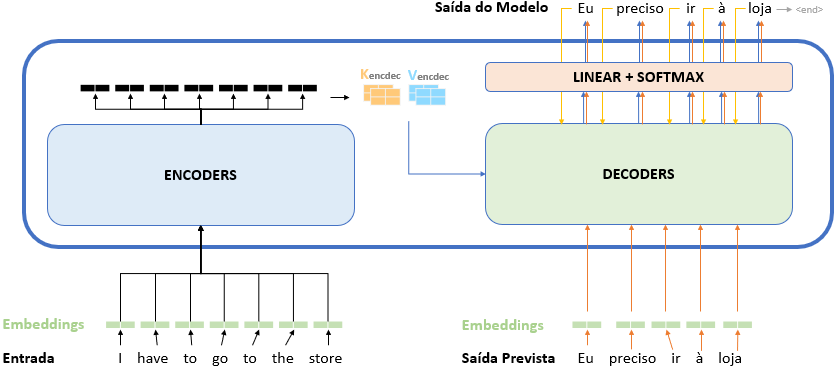
\includegraphics[scale=0.7]
            {Imagens/3.6.4-transformer.png}
    	\end{center}
        \label{img:3.6.4}
    	Fonte: Adaptado de \cite{alammartransformer}.
    \end{figure}

Com isso, a arquitetura \textit{transformer} acaba sendo preferida em diversas tarefas em relação a RNNs e LSTMs, pois as palavras não precisam entrar na rede na sequência original; todas elas são processadas simultaneamente, permitindo a paralelização das operações, o que gera um ganho de performance em termos de velocidade. O mecanismo de atenção é aplicado de forma eficiente, criando uma relação entre as palavras, até mesmo aquelas distantes umas das outras, melhorando a performance no quesito precisão \cite{popel2018}.

Além disso, após cada unidade de atenção e feed-forward, existem camadas de adição e normalização \cite{popel2018}, e o \textit{transformer} adiciona a cada \textit{embedding} um \textit{positional encoding}, que tem o objetivo de manter a relação temporal entre as palavras, ou seja, a rede sabe qual é a sequência original de cada palavra \cite{vaswani2017}. A Figura \ref{img:3.6.5} representa as camadas do \textit{encoder} e \textit{decoder} de uma pilha da arquitetura \textit{transformer}.

\begin{figure}[htb]
    \centering
    \caption{Camadas do \textit{encoder} e \textit{decoder} do \textit{transformer}.}
    \begin{center}
        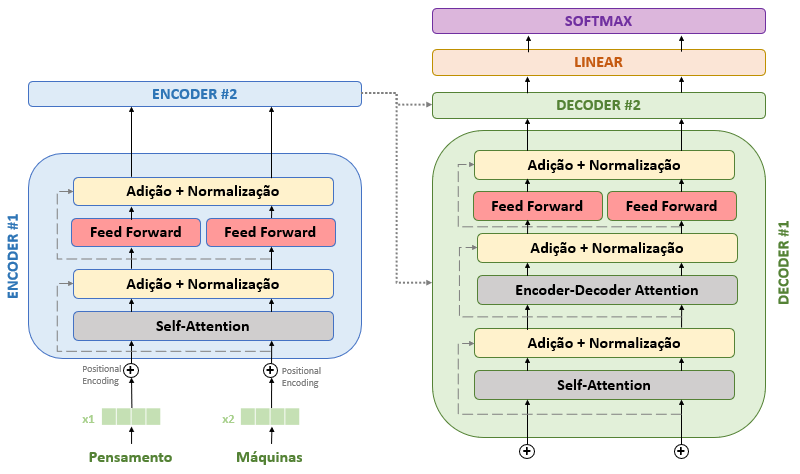
\includegraphics[scale=0.7]
        {Imagens/3.6.5-camadastransformer.png}
    \end{center}
    \label{img:3.6.5}
    Fonte: Adaptado de \cite{alammartransformer}.
\end{figure}
 
%%%%%%%%%%%%%%%%%%%%%%%%%%%%%%%%%%%%%%%%%%%%%%%%%%%%%%%%%%%%%%%%%%%%%%%%%%%%%%%%%%%%%%%%%%%%%%
\section {LLM}

Grandes Modelos de Linguagem (\textit{Large Language Models} ou LLMs) são modelos de inteligência artificial que utilizam técnicas de aprendizado de máquina para entender e gerar linguagem humana. Esses modelos se baseiam em redes neurais profundas e adotam técnicas de processamento de linguagem natural para computar e calcular suas respostas \cite{touvron2023}.

As LLMs utilizam um método denominado aprendizado não supervisionado. Nesse processo, o modelo é alimentado com um grande conjunto de dados (bilhões de palavras e frases) com o objetivo de "aprender" sobre a linguagem \cite{touvron2023}.

À medida que o modelo aprende os padrões de associação entre palavras, ele consegue prever estruturas de frases com base na probabilidade. O resultado final é um modelo capaz de capturar as complexas relações entre palavras e frases \cite{touvron2023}.

Com um vasto conjunto de dados e numerosos cálculos probabilísticos, os LLMs exigem um volume significativo de recursos computacionais. As unidades de processamento gráfico (GPUs) são hardwares criados para lidar com tarefas de processamento complexas e simultâneas, sendo ideais para modelos como os LLMs \cite{strubell2019}.

Para aprimorar a capacidade de um LLM, a arquitetura Transformer absorve eficientemente as dependências e relações contextuais entre os elementos de uma sequência de dados através de seus parâmetros. Esses parâmetros definem limites que são essenciais para analisar o grande volume de dados \cite{naveed2024}.

Com o desenvolvimento do ChatGPT e do GPT-4 (\textit{Generative Pre-trained Transformer}) pela OpenAI, ocorreu uma revolução na percepção sobre os LLMs \cite{openai2024}. Apesar de possuírem desempenho notável, a OpenAI não divulgou detalhes sobre as estratégias de treinamento ou os parâmetros de peso utilizados.

Em resposta, a Meta desenvolveu o modelo denominado LLaMA (\textit{Large Language Model Meta AI}), que é de código aberto e possui tamanhos variados, de 7 bilhões até 405 bilhões de parâmetros. Os autores afirmam que o modelo apresenta desempenho equivalente aos principais modelos, como o GPT-4, e está próximo de atingir o estado da arte em uma variedade de tarefas \cite{touvron2023}. O LLaMA consiste em duas etapas principais:

\begin{itemize}
    \item \textbf{Pré-treinamento}: no qual o modelo é treinado em grande escala usando tarefas simples como a previsão da próxima palavra \cite{llama3}.
    \item \textbf{Pós-treinamento}: no qual o modelo é ajustado para seguir instruções, alinhar-se às preferências humanas e melhorar capacidades específicas (como a codificação) \cite{llama3}.
\end{itemize}

O modelo LLaMA, atualmente na versão 3.3, suporta nativamente multilinguismo, codificação e raciocínio. Seu maior modelo Transformer possui 405B de parâmetros e processa informações em uma janela de contexto de até 128k tokens \cite{llama3}.

Para obter esses resultados, os autores afirmam que um grande modelo de linguagem de alta qualidade precisa de:

\begin{itemize}
    \item \textbf{Dados}: Qualidade e quantidade de dados utilizados tanto no pré-treinamento quanto no pós-treinamento são essenciais. Foi utilizado um corpus de cerca de 15T de tokens multilíngues \cite{llama3}.
    \item \textbf{Escala}: O modelo foi pré-treinado utilizando 3,8 \(\times\) 10\(^{25}\) FLOPs no pré-treinamento. FLOPs ou Operações de Ponto Flutuante representam o número de cálculos de ponto flutuante (adições, multiplicações, etc.) realizados durante o treinamento. A estimativa de FLOPs foi desenvolvida pela OpenAI: \(\text{FLOPs} = 6ND\), onde \(N\) são parâmetros e \(D\) são tokens. O LLaMA 3 possui 400B de parâmetros, resultando em \(6 \times 400 \times 15T = 3,8 \times 10^{25}\) \cite{llama3}.
    \item \textbf{Gerenciamento da complexidade}: Maximizar a capacidade de escalar o processo de desenvolvimento do modelo utilizando o modelo Transformer padrão \cite{vaswani2017}, além de adotar um procedimento de pós-treinamento simples com base em ajuste fino supervisionado (SFT), amostragem de rejeição (RS) e otimização de preferência direta (DPO) \cite{rafailov2024}.
\end{itemize}

Para a criação do modelo LLaMA 3, o corpus multilíngue foi convertido em tokens e pré-treinado para executar a previsão do próximo token. Nesse estágio, o modelo aprende a estrutura da linguagem \cite{llama3}.

O pré-treinamento é realizado em grande escala, utilizando um modelo de 405B de parâmetros em 15,6T de tokens, com uma janela de contexto inicial de 8k tokens. Esse processo é sequencial, aumentando progressivamente a janela de contexto até atingir 128k tokens. O modelo utiliza o algoritmo AdamW com uma taxa de aprendizado de pico de \(8 \times 10^{-5}\), aquecimento linear de 8000 passos e uma programação de taxa de aprendizado decrescente em cosseno até \(8 \times 10^{-7}\) \cite{llama3}.

Os dados do pré-treinamento incluem informações até o final de 2023 obtidas na web. Foram utilizados métodos de desduplicação e mecanismos de limpeza de dados em cada fonte para garantir tokens de alta qualidade, além de remover domínios com conteúdo adulto e informações pessoalmente identificáveis \cite{llama3}.

Um classificador foi desenvolvido para categorizar os tipos de informações contidas nos dados, permitindo a inclusão de categorias específicas. Após vários testes, foi estabelecida a seguinte distribuição de tokens: 50\% de conhecimento geral, 25\% matemáticos e de raciocínio, 17\% de código e 8\% multilíngues \cite{llama3}.

No estágio final do pré-treinamento, sequências longas foram utilizadas para dar suporte às janelas de contexto de até 128k tokens. O treinamento em sequências longas foi evitado inicialmente devido ao aumento quadrático na complexidade computacional das camadas de autoatenção. O comprimento do contexto foi aumentado gradualmente até que o modelo se adaptasse com sucesso \cite{llama3}.

Este processo foi realizado em seis estágios, utilizando aproximadamente 800B de tokens de treinamento. Assim como a OpenAI afirmou, a Meta também relatou que o recozimento melhorou o desempenho dos modelos em até 24\%, embora em algumas versões a melhoria tenha sido insignificante. Os autores afirmmam que modelos com forte capacidade de aprendizado e raciocínio em contexto não necessitam de amostras específicas de treinamento em domínios para obter bom desempenho \cite{llama3}.

O LLaMA 3 utiliza a arquitetura Transformer densa e padrão \cite{vaswani2017}, com atenção de consulta agrupada \cite{ainslie2023} e oito cabeças de chave-valor para melhorar a velocidade de inferência e reduzir o tamanho dos caches durante a decodificação. O modelo também emprega uma máscara de atenção que impede a autoatenção entre diferentes documentos dentro da mesma sequência.

O modelo LLaMA 3 de 405B de parâmetros possui uma arquitetura com 126 camadas e 128 cabeças de atenção, atingindo o tamanho computacionalmente ótimo de acordo com as leis de escala para o orçamento de treinamento da Meta. Essas leis determinam o tamanho ideal do modelo conforme o orçamento computacional \cite{llama3}.

Após o modelo adquirir uma rica compreensão da linguagem, mas ainda não ser capaz de seguir instruções, inicia-se o pós-treinamento. Este estágio utiliza um modelo de recompensa sobre o ponto de verificação pré-treinado com dados de preferência anotados por humanos. Em seguida, os pontos de verificação são ajustados com Ajuste Fino Supervisionado (SFT) em dados de ajuste de instrução e Otimização de Preferência Direta (DPO) \cite{llama3}.

O Ajuste Fino Supervisionado (SFT) é uma etapa de treinamento em modelos AM, especialmente usada em LLMs. Essa etapa ocorre após o treinamento inicial (pré-treinamento) do modelo em um grande conjunto de dados não supervisionados. No SFT, o modelo é ajustado usando um conjunto de dados rotulado e supervisionado, onde há exemplos de entrada e saída esperada. O objetivo é alinhar o modelo com tarefas específicas, reduzindo erros e melhorando seu desempenho em problemas delimitados.

A Otimização de Preferência Direta (DPO) é uma técnica emergente que busca alinhar os modelos diretamente com preferências humanas ou critérios de qualidade especificados. Em vez de ajustar o modelo com base em dados supervisionados ou respostas específicas, a DPO utiliza comparações de preferências humanas (como exemplo, a DPO retornará "Resposta A é melhor que Resposta B"). Com base nessas comparações, o modelo é ajustado para produzir respostas que maximizem a preferência do usuário.

O Modelo de Recompensa (RM) utiliza dados de preferência para gerar pares de respostas (escolhida e rejeitada), além de gerar anotações para edição de respostas. Cada amostra de classificação de preferência possui duas ou três respostas com hierarquia clara (editado > escolhido > rejeitado) \cite{llama3}.

Por fim, o prompt é concatenado com as respostas em uma única linha, embaralhadas aleatoriamente, e então separadas para cálculo de pontuação. Esta abordagem melhora a eficiência do treinamento sem perda de precisão.

Para melhorar ainda mais os modelos de LLM, podem ser utilizadas técnicas como a \textit{Retrieval-Augmented Generation} (RAG). A RAG representa uma inovação significativa na operação dos LLM, pois ajuda a melhorar a precisão e a atualidade das respostas do modelo \cite{lewis2021}.

Diferentemente do fine-tuning, a RAG introduz um sistema intermediário de pesquisa em bases de dados externas, frequentemente implementado como Bases de Dados Vetoriais (VecDBs) \cite{akkiraju2024}.

A eficácia da RAG tem sido demonstrada em vários domínios que exigem informações atualizadas. Por exemplo, Gautier Izacard e Touvron, mostraram que modelos RAG superaram os LLM tradicionais em tarefas de pergunta-resposta de domínio aberto, alcançando uma melhoria de até 30\% em métricas padrão como \textit{Exact Match} e \textit{F1-score} \cite{izacard2021}.

A metodologia RAG fundamenta-se em três componentes técnicos principais: pesquisa vetorial, similaridade vetorial e \textit{re-ranking}, confome a Figura \ref{img:3.7.1}. Estes elementos permitem que o sistema supere a simples correspondência de palavras-chave, possibilitando a identificação do significado semântico das palavras para produzir respostas mais contextualizadas \cite{manning2008}.

\begin{figure}[htb]
    \centering
    \caption{Arquitetura RAG: Geração Aumentada por Recuperação}
    \begin{center}
        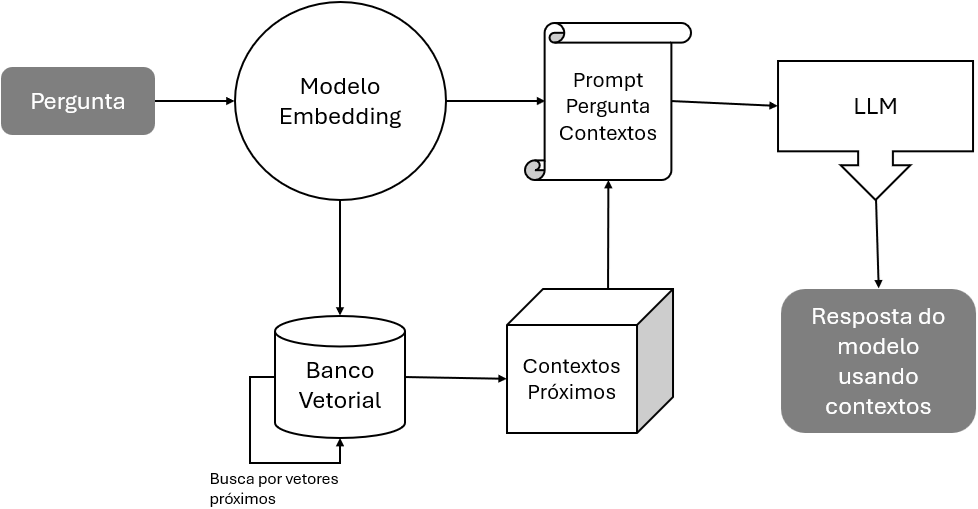
\includegraphics[scale=0.5]
        {Imagens/3.7.1-rag.png}
    \end{center}
    \label{img:3.7.1}
    Fonte: Própria (2024).
\end{figure}

\begin{itemize}
    \item \textbf{Pesquisa vetorial}: Utiliza representações numéricas de alta dimensão para codificar o conteúdo semântico dos textos \cite{mikolov2013a}.
    \item \textbf{Similaridade vetorial}: Aplica métricas matemáticas para quantificar a proximidade semântica entre vetores. As métricas mais comuns da similaridade vetorial são: Similaridade do Cosseno, Distância Euclidiana e Produto Escalar \cite{mikolov2013a}.
    \item \textbf{Re-ranking}: Implementa algoritmos adicionais para ajustar os resultados iniciais da pesquisa, dando maior probabilidade aos mais relevantes \cite{mikolov2013a}.
\end{itemize}

Outra técnica também utilizada para melhorar as respostas de LLMs é a engenharia de \textit{prompt}, que envolve a preparação de estratégias de códigos ou estímulos para gerar respostas características, concisas e proeminentes. Com isso, torna-se uma prática essencial para o aproveitamento máximo das potencialidades dos LLMs \cite{brown2020}.

O \textit{prompt} funciona como uma configuração dos modelos para que uma tarefa possa ser concluída. Não se trata apenas da criação de instruções independentes, mas de uma habilidade que tenha um entrosamento profundo das capacidades e limitações dos LLMs. Existem vários estágios para refinar, repetir e testar continuamente os prompts com base nos resultados obtidos \cite{nascimento2024}.

O \textit{prompt} deve ser descrito de forma clara e precisa, contendo as informações necessárias para que o modelo compreenda a tarefa a ser executada, bem como o formato da resposta esperada. Para alcançar melhor qualidade nos dados extraídos, Zhang afirma que, para modelos LLaMa, os prompts devem ser mantidos pequenos e simples para um melhor entendimento da tarefa \cite{zhang2024}. 

\textit{Prompts} muito longos podem fazer com que os modelos percam informações relevantes. Além disso, a quantidade de amostras fornecidas como exemplos influencia diretamente na qualidade da extração, pois modelos com mais exemplos claros possibilitam uma compreensão mais precisa de como a tarefa deve ser realizada \cite{zhang2024}.

%%%%%%%%%%%%%%%%%%%%%%%%%%%%%%%%%%%%%%%%%%%%%%%%%%%%%%%%%%%%%%%%%%%%%%%%%%%%%%%%%%%%%%%%%%%%%%
\section {RASE}

Com o objetivo de captar informações presentes em regulamentos, estruturar o processo de conversão dessas regras para uma linguagem computacional e aplicar a verificação automática de modelos em grande escala, Hjelseth desenvolveu as metodologias Tx3 e RASE \cite{hjelseth2015}. 

A metodologia Tx3 propõe três ações a serem realizadas conforme a classificação das informações presentes nos regulamentos: 

\begin{itemize}
    \item \textbf{Transcrever (T1)}: Deve ser aplicada para instruções que podem ser diretamente transcritas em regras computáveis; 
    \item \textbf{Transformar (T2)}: Deve ser aplicada para instruções que necessitam ser reestruturadas ou reescritas de forma a preservar o sentido original;
    \item \textbf{Transferir (T3)}: Deve ser aplicada quando os requisitos são expressos de maneira imprecisa, sem conexão clara entre os objetivos do regulamento e os indicadores. Nestes casos, é necessária a análise de um profissional especializado.
\end{itemize}

Após a classificação do texto original, os elementos classificados como T1 e T2 são reescritos e submetidos à metodologia RASE. A metodologia RASE, baseada em conceitos semânticos, transforma documentos normativos em regras bem definidas, utilizáveis em softwares baseados em BIM \cite{hjelseth2011}. O processo consiste na identificação de quatro operadores lógicos:

\begin{itemize}
    \item \textbf{Requisito (R)}: Expressa o dever associado, frequentemente identificado pelo imperativo “deve”. Por exemplo, na frase “Toda rota acessível de espaço privado deve ser provida de iluminação natural ou artificial com nível mínimo de iluminância de 150 lux medidos a 1,00 m do chão”, o requisito é: “deve ser provida de iluminação natural ou artificial com nível mínimo de iluminância de 150 lux”.
    \item \textbf{Aplicabilidade (A)}: Identifica a quem ou ao que o requisito se aplica. No exemplo anterior, a aplicabilidade é: “rota acessível”.
    \item \textbf{Seleção (S)}: Indica um subconjunto da aplicabilidade. No exemplo, a seleção é: “de espaço privado”;
    \item \textbf{Exceção (E)}: Define os elementos excluídos da regra. Completando o exemplo anterior com a norma “São aceitos níveis inferiores de iluminância para ambientes específicos, como cinemas, teatros ou outros, conforme normas técnicas específicas.”, a exceção é: “níveis inferiores para cinemas, teatros e outros”, pois isso não se aplica a regra. 
\end{itemize}

Para facilitar a visualização, utiliza-se um sistema de cores, onde de costume é utilizado: Requisitos (azul), Aplicabilidade (verde), Seleção (vermelho) e Exceção (laranja). Cada operador identificado é associado a atributos específicos:
\begin{itemize}
    \item \textbf{Objeto}: Termos padronizados, como “escada” ou “corrimão”.
    \item \textbf{Propriedade (A)}: Termos classificados, como “nível de iluminância” ou “sistema de segurança”.
    \item \textbf{Comparador}: Pode ser maior, menor, igual, diferente, entre outros.
    \item \textbf{Valor}: Valores numéricos, unidades ou descrições.
    \item \textbf{Unidade}: Tipo de unidade do valor numérico caso exista. 
\end{itemize}

Como exemplo, considere o texto da norma NBR 9050: “A inclinação transversal da superfície deve ser de até 2\% para pisos internos e de até 3\% para pisos externos. A inclinação longitudinal da superfície deve ser inferior a 5\%. Inclinações iguais ou superiores a 5\% são consideradas rampas e, portanto, devem atender a 6.6.” 

Aplicando a metodologia Tx3 e RASE:

\begin{itemize}
    \item \textbf{Tx3 (Transcrever)}:
    \begin{itemize}
        \item Pisos internos devem ter inclinação transversal menor ou igual a 2\%;
        \item Pisos externos devem ter inclinação transversal menor ou igual a 3\%;
        \item Pisos internos devem ter inclinação longitudinal menor do que 5\%;
        \item Pisos externos devem ter inclinação longitudinal menor do que 5\%;
        \item Pisos com inclinação longitudinal maior ou igual a 5\% são considerados rampas e devem atender a 6.6;
    \end{itemize}

    \item \textbf{RASE (Operadores)}:
    \begin{itemize}
        \item A\{Pisos\} S\{internos\} R\{devem ter inclinação transversal menor ou igual a 2\%\};
        \item A\{Pisos\} S\{externos\} R\{devem ter inclinação transversal menor ou igual a 3\%\};
        \item A\{Pisos\} S\{internos\} R\{devem ter inclinação longitudinal menor do que 5\%\};
        \item A\{Pisos\} S\{externos\} R\{devem ter inclinação longitudinal menor do que 5\%\};
        \item A\{Pisos\} E\{com inclinação longitudinal maior ou igual a 5\% são consideradas rampas\} R\{devem atender a 6.6\};
    \end{itemize}
\end{itemize}

Por fim, após obter os operadores RASE é gerado o atributo de cada um dos operadores, como mostra a Figura \ref{img:3.8.1}.

\begin{figure}[htb]
    \centering
    \caption{Utilização da metodologia RASE na NBR 9050}
    \begin{center}
        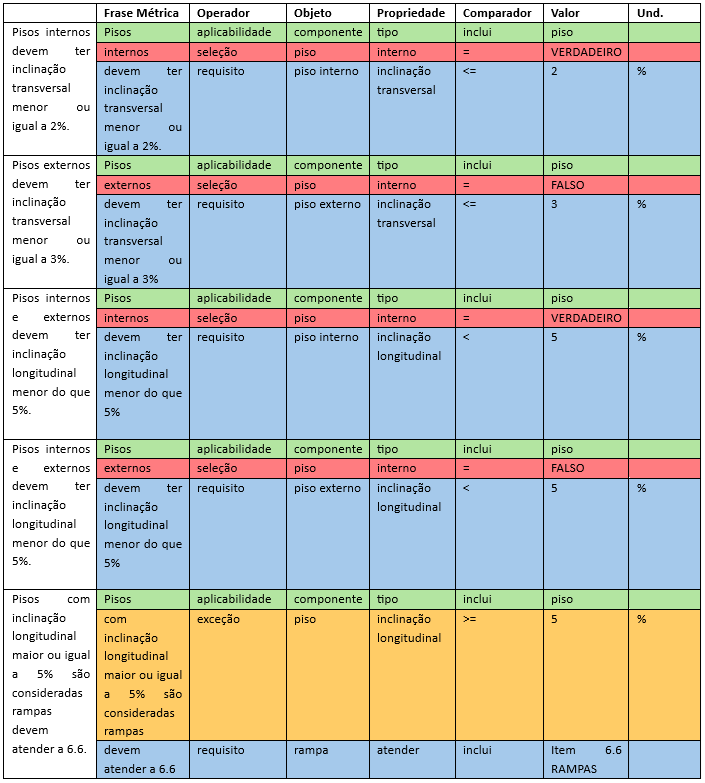
\includegraphics[scale=0.8]
        {Imagens/3.8.1-rase.png}
    \end{center}
    \label{img:3.8.1}
    Fonte: Própria (2024).
\end{figure}

%%%%%%%%%%%%%%%%%%%%%%%%%%%%%%%%%%%%%%%%%%%%%%%%%%%%%%%%%%%%%%%%%%%%%%%%%%%%%%%%%%%%%%%%%%%%%%

\section {Trabalhos Relacionados}

A integração do BIM com tecnologias de inteligência artificial generativa (IAG), como o ChatGPT, tem sido pouco explorada no setor de Arquitetura, Engenharia e Construção (AEC). Este tema abrange aplicações práticas, frameworks inovadores, desafios e possibilidades futuras, sendo objeto de estudo de diversos trabalhos recentes.

Um dos estudos analisados aborda a integração do BIM com modelos de IAG, como o ChatGPT e o Bard. Este artigo identifica que a utilização dessas tecnologias visa otimizar processos como design e tomada de decisão \cite{rane2023}. No entanto, os autores destacam desafios, como a falta de padronização de dados, deficiências em segurança e a necessidade de capacitação de profissionais do setor \cite{rane2023}. Além disso, os modelos generativos enfrentam dificuldades em interpretar a semântica complexa de dados BIM, além de problemas gerais, como alta demanda computacional e falta de diretrizes éticas \cite{rane2023}. Em resposta a essas lacunas, os pesquisadores propõem um framework voltado à otimização de processos, redução de custos e tempo, e à facilitação da adoção de IA por meio de interfaces mais intuitivas \cite{rane2023}.

Outro estudo relevante trata do desenvolvimento de um chatbot, denominado JULE, projetado para gerentes de obras \cite{lin2023}. Este modelo utiliza BIM e técnicas de Processamento de Linguagem Natural (PLN) para fornecer informações precisas e em tempo real no canteiro de obras. O chatbot permite que os usuários consultem dados como dimensões de componentes estruturais e ferramentas necessárias de forma ágil e intuitiva, eliminando a dependência de interfaces convencionais \cite{lin2023}. A abordagem proposta demonstrou alta precisão na identificação de intenções e na recuperação de informações essenciais, melhorando a adoção de sistemas baseados em BIM e promovendo maior eficiência no gerenciamento de obras \cite{lin2023}.

Um trabalho adicional investigou a aplicação de LLMs, como GPT-3.5 e GPT-4, em projetos BIM voltados à segurança \cite{sammou2024}. Os autores realizaram testes com 385 questões de múltipla escolha de exames certificados pela BCSP, abrangendo áreas como gestão de sistemas de segurança, identificação de perigos e ergonomia \cite{sammou2024}. Utilizando técnicas de engenharia de \textit{prompt}, como \textit{Prompt Direct}, \textit{Prompt Chain-of-Thought} e \textit{Prompt Few-Shot}, os modelos foram avaliados em termos de precisão e consistência. Os resultados indicaram que o GPT-4 alcançou 84,6\% de precisão, enquanto o GPT-3.5 obteve 73,8\%. Apesar do bom desempenho em áreas como gerenciamento de sistemas e controle de perigos, ambos os modelos apresentaram dificuldades em responder questões relacionadas a emergências e cálculos matemáticos \cite{sammou2024}. A pesquisa destacou o potencial desses modelos, mas também a necessidade de melhorias para evitar informações imprecisas ou enviesadas \cite{sammou2024}.

Por fim, outro estudo explorou diferentes técnicas de engenharia de prompt para otimizar a utilização de LLMs no setor AEC. Os autores identificaram que métodos genéricos de interação limitam a eficácia desses modelos, resultando em saídas desalinhadas com as necessidades do setor \cite{samsami2024}. Problemas como confiabilidade, adaptação a regulamentações e aceitação no setor também foram identificados como barreiras. A pesquisa coletou técnicas de prompt eficazes, como prompts instrucionais e baseados em restrições, e testou essas abordagens em projetos reais \cite{samsami2024}. Os resultados mostraram que prompts específicos reduziram erros em cronogramas e melhoraram o reconhecimento de perigos. Apesar disso, limitações como alucinações do modelo para tarefas complexas e a necessidade de validação externa ainda persistem \cite{samsami2024}.

Os trabalhos analisados fornecem uma visão abrangente sobre o estado da arte na integração de LLMs e BIM no setor AEC. Embora avanços significativos tenham sido alcançados, desafios importantes, como a interpretação semântica de dados BIM, segurança e a adaptação de LLMs às demandas específicas do setor, ainda necessitam de soluções mais robustas. Assim, este campo continua a ser promissor para futuras pesquisas e inovações.

\subsection{Análise dos Trabalhos Relacionados}

A integração de BIM com LLMs e IA generativa no setor AEC tem mostrado avanços, mas também apresenta desafios. Um estudo identificou a utilização de tecnologias como ChatGPT e Bard para otimizar processos, como design e tomada de decisão. No entanto, as dificuldades incluem a falta de padronização de dados, questões de segurança e a complexidade semântica dos dados BIM \cite{rane2023}. O uso de LLMs aqui é bom devido à sua capacidade de processar grandes volumes de dados e fornecer \textit{insights} valiosos, mas a interpretação semântica continua sendo uma limitação.

Outro estudo sobre o chatbot JULE, que usa BIM e PLN, mostrou avanços na eficiência do gerenciamento de obras, permitindo consultas rápidas no canteiro. No entanto, como o modelo depende de dados BIM bem estruturados, as falhas na semântica e na adaptação dos dados para o modelo ainda representam uma barreira \cite{lin2023}. Mesmo assim, o uso de LLMs para interpretar regras e padrões regulatórios é promissor devido à sua agilidade na recuperação de informações.

Um estudo com LLMs como GPT-3.5 e GPT-4 aplicados a segurança em BIM demonstrou precisão significativa, mas também dificuldades em questões complexas como emergências e cálculos. A limitação aqui está na falta de confiabilidade para questões mais técnicas, e embora os LLMs possam interpretar normas e regulamentos, é necessário garantir maior precisão e evitar informações enviesadas \cite{sammou2024}.

Além disso, a pesquisa sobre técnicas de engenharia de prompt para otimizar LLMs no setor AEC destacou que prompts genéricos não são eficazes. O uso de prompts mais específicos melhorou a precisão, mas problemas como alucinações do modelo e a necessidade de validação externa persistem \cite{samsami2024}. A adaptação dos modelos às regulamentações específicas do setor é crucial, e o uso de LLMs para interpretar regras regulatórias se mostra útil, mas ainda exige ajustes finos e validação.